\chapter{Descripción del mecanismo de conexión al SGBD}
MongoDB cuenta con drivers para una multitud de lenguajes, y Atlas provee lineas de conexión generadas automáticamente para aplicaciones JavaScript y Python. Para conectarnos a nuestro clúster desde una aplicación Python seguiremos los siguientes pasos:

\begin{enumerate}
  \item Desde una terminal, instalamos con Pip el driver Pymongo:
  \begin{lstlisting}
  python -m pip install pymongo[snappy,gssapi,srv,tls]
  \end{lstlisting}

  \item Abrimos la shell de Python, importamos el paquete y comprobamos qué versión tenemos:
  \begin{lstlisting}
  > python
  > import pymongo
  > pymongo.version
  \end{lstlisting}

  \item Desde Atlas, elegimos en nuestro clúster la opción conectar. Igual que para conectarnos con Compass, introduciremos nuestra IP y usuario.

  \item Para el método de conexión escogemos conectar a aplicación. Desde el desplegable, escogemos Python y nuestra versión de Pymongo, la cual hemos consultado en el paso 2.
    \begin{figure}[!h]
      \centering
        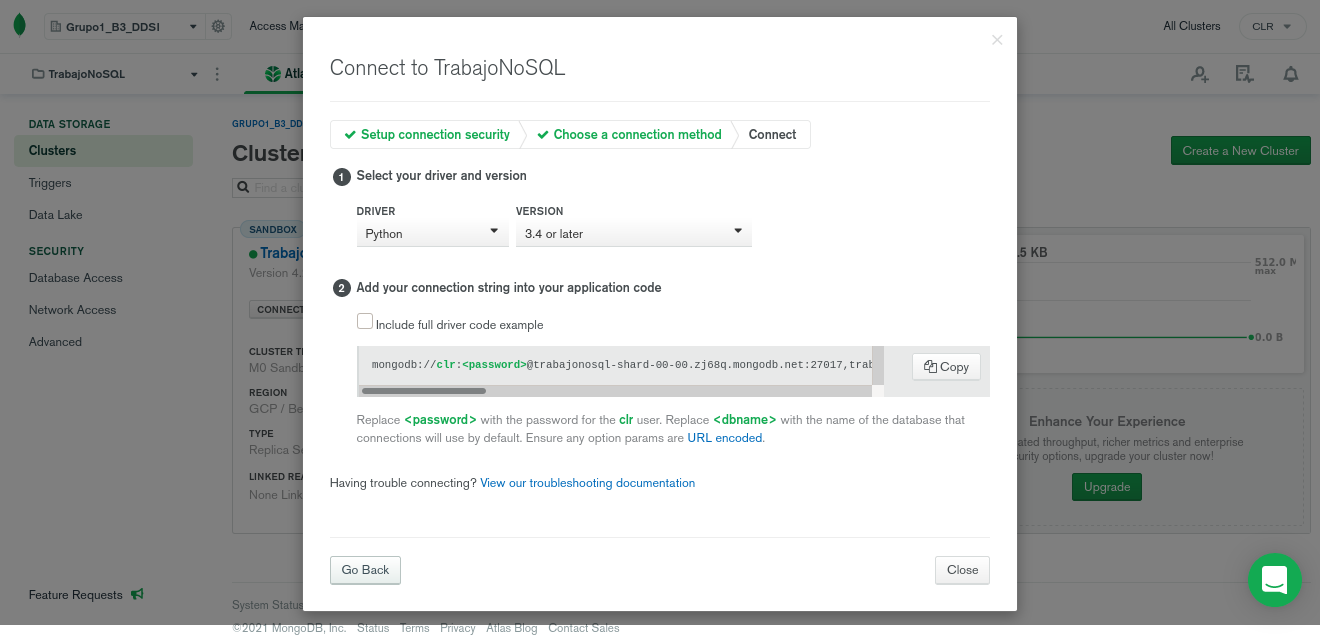
\includegraphics[scale=0.2]{conn.png}
    \end{figure}

  \item Importamos Pymongo y MongoClient a nuestro programa Python con el siguiente comando
  \begin{lstlisting}
  from pymongo import MongoClient
  \end{lstlisting}

  \item En la línea que nos da Atlas (string de conexión), sustituímos \texttt{<password>} por nuestra contraseña, y \texttt{<dbname>} por la base de datos por defecto que queramos.

  \item Una vez hemos la string de conexión tiene nuestra contraseña y base de datos, la pegamos dentro de la función MongoClient() en nuestro programa Python de la siguiente manera, sustituyendo la línea punteada:
  \begin{lstlisting}
  client = MongoClient('- - - - - - - - - - - - - - - -')
  \end{lstlisting}

\end{enumerate}
